% Created 2015-01-30 Fre 23:42
\documentclass[11pt, a4paper,titlepage]{article}
\usepackage[utf8]{inputenc}
\usepackage[T1]{fontenc}
\usepackage{fixltx2e}
\usepackage{graphicx}
\usepackage{longtable}
\usepackage{float}
\usepackage{wrapfig}
\usepackage{soul}
\usepackage{textcomp}
\usepackage{marvosym}
\usepackage{wasysym}
\usepackage{latexsym}
\usepackage{amssymb}
\usepackage{hyperref}
\tolerance=1000
\usepackage[left=2.35cm, right=3.35cm, top=3.35cm, bottom=3.35cm]{geometry}
\usepackage[utf8]{inputenc}
\usepackage[english]{babel}
\usepackage{graphicx}
\usepackage{titlesec}
\usepackage{chemfig}
\usepackage{tocbibind}
\providecommand{\alert}[1]{\textbf{#1}}

\title{}
\author{Cedric Lood}
\date{\today}
\hypersetup{
  pdfkeywords={},
  pdfsubject={},
  pdfcreator={Emacs Org-mode version 7.9.3f}}

\begin{document}



\setlength{\parskip}{0pt}%
\setlength{\parindent}{0pt}%
\renewcommand{\thesubsubsection}{\alph{subsubsection}.)}
\begin{titlepage}
  \begin{center}
    
    
\includegraphics[scale=1.5]{Figures/kuleuven_logo.pdf}~\\[4.5cm]
    
    \textsc{\Large Basics of biological chemistry}\\[0.5cm]
    
    % Title
    \rule{\linewidth}{0.3mm}\\[0.4cm]
    {\huge \bfseries Assignment} \\[0.4cm]
    {\large January 2015 Finals} \\[0.4cm]
    \rule{\linewidth}{0.3mm}\\[1.5cm]
    
    % Author and supervisor
    \begin{minipage}{0.4\textwidth}
      \begin{flushleft} \large
        \emph{Author:}\\
        Cedric \textsc{Lood}\\
      \end{flushleft}
    \end{minipage}
    \begin{minipage}{0.4\textwidth}
      \begin{flushright} \large
        \emph{Supervisors:} \\
        Prof. J. \textsc{Vanderleyden}\\
        dr. H. \textsc{Steenackers}\\
        Prof. B. \textsc{Sels}\\
        Prof. J. \textsc{Vanderleyden}
      \end{flushright}
    \end{minipage}
    
    \vfill
    
    % Bottom of the page
    {\large \today}
    
  \end{center}
\end{titlepage}

\setcounter{tocdepth}{3}
\tableofcontents
\clearpage

\section{Questions from Prof. J. Vanderleyden – dr. H. Steenackers}
\label{sec-1}

Note: reference material for this part mostly come from the
recommended class book \cite{BioChemBlei}
\subsection{Chemical reaction equation}
\label{sec-1-1}


Consider the following reaction: (NH$_{4}$)$_{2}$CO$_{3}$ +  Zn(NO$_{3}$)$_{2}$ →  NH$_{4}$NO$_{3}$ + ZnCO$_{3}$
\subsubsection{Balance the equation}
\label{sec-1-1-1}

(NH$_{4}$)$_{2}$CO$_{3}$ +  Zn(NO$_{3}$)$_{2}$ →  2 NH$_{4}$NO$_{3}$ + ZnCO$_{3}$
\subsubsection{Reactants and products}
\label{sec-1-1-2}

\texttt{Q:} Name all reactants and reaction products.

\texttt{A:}
\begin{itemize}
\item (NH$_{4}$)$_{2}$CO$_{3}$ : Ammonium Carbonate
\item Zn(NO$_{3}$)$_{2}$ : Zinc Nitrate
\item NH$_{4}$NO$_{3}$ : Ammonium Nitrate
\item ZnCO$_{3}$ : Zinc Carbonate
\end{itemize}
\subsubsection{Lewis structure, VESPR}
\label{sec-1-1-3}

\texttt{Q:} Construct the Lewis structures of the polyatomic ions you recognize
and predict their molecular structure using the VSEPR theory.

\texttt{A:}
\begin{itemize}
\item Lewis Structure of the ions:
\end{itemize}
\renewcommand{\arraystretch}{1.5}
\begin{tabular}{ c | c | c | c}
Ammonium & Carbonate & Zinc & Nitrate  \\
\hline
\chemfig{N^{+}(-[:0]H)(-[:90]H)(-[:180]H)(-[:270]H)} &
\chemfig{\lewis{3:5:,O}=C(-[1]\lewis{3:1:7:,O}^{-})(-[7]\lewis{1:7:5:,O}^{-})} &
\chemfig{\lewis{0.4.,Zn^{2+}}} &
\chemfig{\lewis{3:5:,O}=N^{+}(-[1]\lewis{3:1:7:,O}^{-})(-[7]\lewis{1:7:5:,O}^{-})}\\
\end{tabular}

\begin{itemize}
\item Molecular structure prediction:
\end{itemize}
\renewcommand{\arraystretch}{1.5}
\begin{tabular}{ c | c | c | c}
Ammonium & Carbonate & Zinc & Nitrate  \\
\hline
\chemfig{N^{+}(-[2]H)(-[5]H)(<[6]H)(<:[7]H)} &
\chemfig{O=C(-[1]O^{-})(-[7]O^{-})} &
\chemfig{Zn^{2+}} &
\chemfig{O=N^{+}(-[1]O^{-})(-[7]O^{-})}\\
\end{tabular}
\subsubsection{Oxidation states}
\label{sec-1-1-4}

\texttt{Q:} Determine the oxidation state of all the atoms in all the
compounds. Is this an oxidation-reduction reaction?

\texttt{A:} Ammonium Carbonate and Zinc Nitrate (the reactants) are very
soluble in water and will thus move freely as charged ions. The Zinc
and Carbonate ions will precipitate. The reaction is not an
oxydo-reduction as shown by the details below:

\begin{itemize}
\item Zn(NO$_{3}$)$_{2}$ each O are -2, N is +5, (NO3$^{-}$)$_{2}$ is -2, and Zn is +2
\item (NH$_{4}$)$_{2}$CO$_{3}$ N is -3, each H are +1, and (NH$_{4}$)$_{2}$ is
     +2. C is +4 and each O is -2, and (CO$_3$)$^{\mathrm{-2}}$ is -2.
\item NH$_{4}$NO$_{3}$ for NH$_{4}$, the oxidation state is +1, and for NO$_{3}$
  it's -1
\item ZnCO$_{3}$ for Zn, the oxidation is +2, and it's -2 for CO$_3$
\end{itemize}
\subsubsection{Mass}
\label{sec-1-1-5}

\texttt{Q:} How many grams of ZnCO3 can be prepared from 400g Zn(NO3)2 by
using sufficient(NH4)2CO3?

\texttt{A:} Let's start by computing the molecular weight of the 2 reactants:

\begin{description}
\item[Molecular weigth of Zn(NO$_{3}$)$_{2}$] 189.36 g/mol
\item[Molecular weigth of (NH$_{4}$)$_{2}$CO$_{3}$] 96.09 g/mol
\end{description}

Given that there are 400g of Zn(NO$_{3}$)$_{2}$, we can calculate the
number of moles of reactant (and ignore that of (NH$_{4}$)$_{2}$CO$_{3}$
since it is in excess):

\begin{description}
\item[Moles of Zn(NO$_{3}$)$_{2}$] 400 g / 189.36 g/mol = 2.11237 moles
\end{description}

From this last figure, we can infer that the number of moles of
ZnCO$_{3}$ will be 2.11237. Given the molecular mass of ZnCO$_{3}$, we can
compute the amount of ZnCO$_{3}$ produced to be: 2.11237 mol * 125.3889
g/mol = 264.87 g.
\subsection{DNA sequence analysis}
\label{sec-1-2}


The following diagram shows part of a template DNA strand, with
sections X,Y and Z being the exons of a gene:


\begin{verbatim}
5'                        3'
GTA GGT TGT ATC GAT GGT CAT
---     -------         ---
 X         Y             Z
\end{verbatim}
\subsubsection{DNA Replication}
\label{sec-1-2-1}

\texttt{Q:} What is the corresponding sequence on the new daughter strand
made from the given parent strand during replication?

\texttt{A:} Given the principle of base pairing, we can determine the daughter
sequence to be:


\begin{verbatim}
5'                        3'
GTA GGT TGT ATC GAT GGT CAT
CAT CCA ACA TAG CTA CCA GTA
3'                        5'
\end{verbatim}
\subsubsection{Translated Protein}
\label{sec-1-2-2}

\texttt{Q:} What polypeptide sequence will be synthesized from the given template
DNA? Give a short overview of the different processes (and enzymes)
involved in the synthesis of polypeptides from template DNA. Where in
the cell do these processes take place?

\texttt{A:} The synthesized polypeptide will consist of the amino acids
\texttt{Met-Asp-Thr-Tyr} (corresponding mRNA: \texttt{5'AUGGAUACAUAC}). Since it is
mentioned that exons are present, we can assume the translation will
take place with the eukaryotic machinery. It will thus consist of the
following general steps:

\begin{itemize}
\item Transcription: In the nucleus, the RNA Polymerase II will be
  recruited and will bind to the promoter of the gene. It will
  produce, by moving in the 5' to 3' direction, a pre-messenger RNA
  which will be identical to the DNA template sequence (with the
  exception that Uracyl will be used instead of Thymine, and also the
  addition of a 5' CAP). That messenger RNA will then be processed by
  the spliceosome, which will remove the introns, and a Poly-A tail
  will also be added at the 3' end of the mRNA. The mRNA is then
  ready to go outside of the nucleus to be translated.
\item Translation: the mRNA leaves the nucleus and passes through the
  reticulated ER where it will be captured by a ribosome that will
  either bind to the ER or not depending on the signal encoded in the
  mRNA. It will then start scanning for a start codon in the
  mRNA. From that point on, the synthesis of a polypeptide will be
  accomplished by reading 3 base pairs at a time and pairing these 3
  with the correct tRNA. After that, the polypeptide will either be
  processed further and sent to the golgi apparatus, or will remain in
  the cytosol.
\end{itemize}
\subsubsection{Mutated exon}
\label{sec-1-2-3}

\texttt{Q:} What polypeptide sequence will be synthesized if the ATC in exon
Y is mutated to TTC? What polypeptide sequence will be synthesized if
the ATC in exon Y is mutated to ATG? Which of those substitution
mutations is likely to be more harmful? Why?

\texttt{A:} Here are the new sequences with mutated exons:

\begin{itemize}
\item TGTATC -> TGTTTC : the resulting polypeptide will be \texttt{Met-Glu-Thr-Tyr}
\item TGTATC -> TGTATG : the resulting polypeptide will be \texttt{Met-His-Thr-Tyr}
\end{itemize}

The second mutation would be the most disruptive. Indeed the original
Aspartate would be negatively charged in the physiological condition,
and the Glutamate would also be negatively charged, the only
difference between the 2 is then an additional CH2 group in the side
chain. Histidine on the the other hand is neutral in physiological
conditions, its side chain is also significantly larger/bulkier due to
the aromatic ring.
\subsubsection{Interactions with antibiotics}
\label{sec-1-2-4}

\texttt{Q:} Which steps in polypeptide synthesis are affected by resp. the
macrolide antibiotics and the tetracycline antibiotics?

\texttt{A:} Both substance have the capabilities to inhibit the synthesis of
proteins by affecting ribosomal activity \cite{AntibioticsRibosomeEffect}. 

\begin{itemize}
\item Macrolide : prevents peptidyltransferase from linking the peptide
  from the tRNA to the growing polypeptide chain.
\item Tetracycline : this one functions by preventing the binding of tRNA
  to mRNA in the ribosome.
\end{itemize}
\subsubsection{Comparison of error rates}
\label{sec-1-2-5}

\texttt{Q:} The error rate in RNA synthesis is much higher than the error rate
of DNA replication. What is the origin of this difference? Motivate
why this is not a serious problem.

\texttt{A:} DNA being the central repository of the genetic information for
an organism, the fidelity of the DNA replication is required to ensure
the continuity of the species and its viability accross multiple
generation. The cell needs thus enforce a high fidelity of the
replication process through an extensive proof reading system. On the
other hand, there is no proof reading for transcription. Whenever an
incorrect mRNA is transcribed, the effect are very local and
temporary, indeed there is no real harm in producing a couple of
non-functioning mRNA or proteins that will eventually be degraded by
the cell.
\subsection{tRNA 3D-Structure}
\label{sec-1-3}

\texttt{Q:} All tRNA molecules have a particular 3D-structure. Which
functional groups and which chemical bonds/interactions contribute to
this particular structure? Why is this particular structure of
importance for the biological function?

\texttt{A:} Below is a representation of a tRNA structure
\cite{tRNA-Phe}. The structure of the tRNA contains a couple of loops
and contains parts with base pairing (hydrogen bonds). This structure
is critical for the correct capture, processing, and release of the
tRNAs by the ribosomes. Couple of important sections can be identified
that are common to tRNAs and critical to their function :

\begin{itemize}
\item Anticodon arm (blue): that loop will contain the anticodon (black)
  which will base pair with the mRNA codon.
\item Acceptor stem (purple): which is the attachment site of the amino
  acids.
\item T-Arm (green): that region is a special recognition site for the
  ribosome. It allows a tRNA-ribosome complex to form and translation
  to proceed.
\end{itemize}

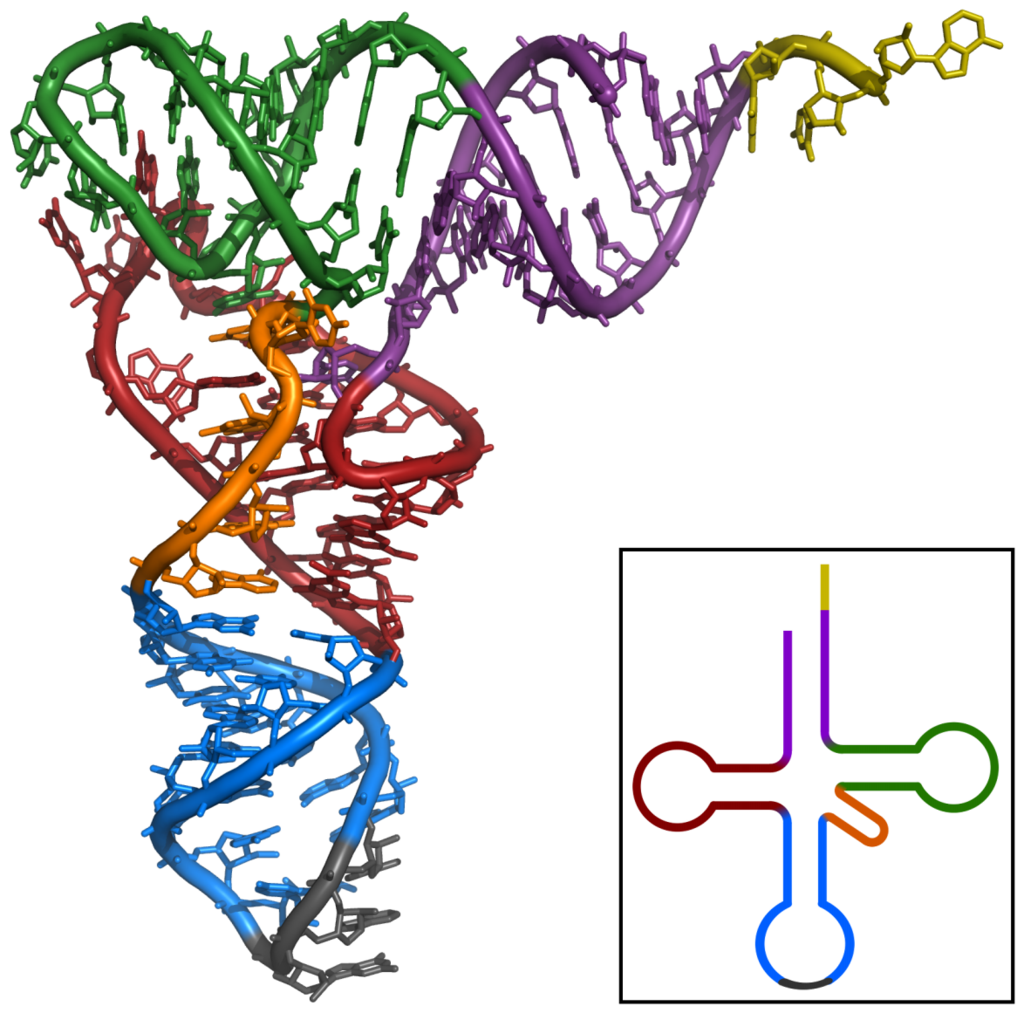
\includegraphics[width=10cm]{./Figures/TRNA-Phe_yeast.png}
\section{Questions from Prof. B. Sels}
\label{sec-2}

Note: reference material for this part mostly come from the
recommended class book \cite{BioChemBlei}
\subsection{Biopolymer organisation}
\label{sec-2-1}

\texttt{Q:} The course and the textbook systematically organize four important
biopolymers mainly according to their chemical structure. Attempt a
complete reorganization of the various biopolymer structures (and
subfamilies!) according to the following three physiological
functions: energy, structure, and communication. Explain the
physiological function of each biopolymer type with regard to its
chemical structure and/or physical properties.

\texttt{A:} The fours main categories of polypeptide consist of the
carbohydrates, the nucleic acids, the proteins (polypeptides), and the
lipids. Here is my attempt at reorganizing them based on the following
categories:
\subsubsection{Energy}
\label{sec-2-1-1}

\begin{itemize}
\item Carbohydrates for short term storage of energy, either for
  immediate release of energy (glucose, galactose, and other monomers
  of C6H12O6), or for midterm storage of energy (Polysaccharide
  glycogen).
\item Lipids can be used in a triglyceride form to store energy for the
  long term.
\item The universal energy conveyor of the cellular life is ATP, which is
  a triphosphated adenosine (nucleic acid).
\end{itemize}
\subsubsection{Structure}
\label{sec-2-1-2}

\begin{itemize}
\item Phospholipids for the cell membrane, cholesterol for its
  fluidity.
\item Fibrous proteins are used to form the exoskeletton and the
  misc filaments in the cell (Actin, Tubulin, etc)
\item Polysaccharides can be used for structure as well, for example as
  cellulose for the rigidity of the plants, or as chitin for the
  exosqueleton of the insects.
\end{itemize}
\subsubsection{Communication}
\label{sec-2-1-3}

\begin{itemize}
\item DNA is the central repository of information for the
  organism genetic makeup, which is passed on through the
  generations.
\item RNA is the intermediate messenger for the translation of
  proteins.
\item Modified amino acids are involved in communication too (eg Thyroxine
  and Melatonin).
\item A host of membrane proteins that help recognizing and process
  signals are found on most cells.
\item Neurotransmitters that carry signal from one neurons' synapses to
  another can be divided in 3 broad constitutive categories, which
  include amino acids, peptides, and monoamines.
\end{itemize}
\subsection{Chemical structure of proteins and proteins separation}
\label{sec-2-2}

\texttt{Q:} Draw the chemical structure of the following two oligopeptide
structures, a) Gln-Ser-Lys-Lys-Ser and b) Cys-Asp-Asp-Glu-Lys,
determine its net charge in physiological conditions. How would you
separate the two peptides ?  

\texttt{A:} These are the chemical structures of:
\begin{itemize}
\item Gln-Ser-Lys-Lys-Ser

  \setatomsep{25pt}
  \chemfig{NH3^{+}-C(-[2]H)(-[6]CH2(-[6]CH2(-[6]C(=[7]O)(-[5]NH2))))-C(=[2]O)-N(-[6]H)-C(-[2]H)(-[6]CH2(-[6]OH))-C(=[2]O)-N(-[6]H)-C(-[2]H)(-[6](CH2(-[6]CH2(-[6]CH2(-[6]CH2(-[6]NH3^{+}))))))-C(=[2]O)-N(-[6]H)-C(-[2]H)(-[6](CH2(-[6]CH2(-[6]CH2(-[6]CH2(-[6]NH3^{+}))))))-C(=[2]O)-N(-[6]H)-C(-[2]H)(-[6]CH2(-[6]OH))-COO^{-}}
\item Cys-Asp-Asp-Glu-Lys

  \setatomsep{25pt}
  \chemfig{NH3^{+}-C(-[2]H)(-[6]CH2(-[6]SH))-C(=[2]O)-N(-[6]H)-C(-[2]H)(-[6]CH2(-[6]COO^{-}))-C(=[2]O)-N(-[6]H)-C(-[2]H)(-[6]CH2(-[6]COO^{-}))-C(=[2]O)-N(-[6]H)-C(-[2]H)(-[6]CH2(-[6]CH2(-[6]COO^{-})))-C(=[2]O)-N(-[6]H)-C(-[2]H)(-[6](CH2(-[6]CH2(-[6]CH2(-[6]CH2(-[6]NH3^{+}))))))-COO^{-}}
\end{itemize}

Under physiological conditions (ie, pH around 7.35), these would be
the net charge on each polypeptide:

\begin{itemize}
\item Gln-Ser-Lys-Lys-Ser: net charge is +2

  \chemfig{\chemabove{NH3}{\scriptstyle\oplus}-Gln-Ser-\chemabove{Lys}{\scriptstyle\oplus}-\chemabove{Lys}{\scriptstyle\oplus}-Ser-\chemabove{COO}{\ominus}}
\item Cys-Asp-Asp-Glu-Lys: net charge is -2

  \chemfig{\chemabove{NH3}{\scriptstyle\oplus}-Cys-\chemabove{Asp}{\ominus}-\chemabove{Asp}{\ominus}-\chemabove{Glu}{\ominus}-\chemabove{Ly}{\scriptstyle\oplus}-\chemabove{COO}{\ominus}}
\end{itemize}

Separation of both proteins can thus be achieved by ion exchange
chromatography since they both have quite a distinct charge
\cite{BioChemPrinciples}. For example, we could use anion exchange
chromatography, which would capture the negatively charged
polypeptide, and let the positively charged one pass through. The
former could then be recovered later on by washing away the column.
\subsection{Chemical structure of disaccharides}
\label{sec-2-3}

\texttt{Q:} Draw the chemical structure of the following disaccharides: a)
the $\beta$-anomer of $\alpha$(1→6)galactoglucose and b)
$\beta$,$\alpha$(1→2)glucofructose.

\texttt{A:} These are the chemical structure of:
\begin{itemize}
\item $\beta$-anomer of $\alpha$(1→6)galactoglucose
\end{itemize}

Beta anomers have a cis relationship between the CH$_{2}$OH group on
the C$_{1}$ and the OH group on the C$_{6}$. This helps us determine the
structure of the monosaccharides galactose and glucose. The
polymerisation is achieved through an $\alpha$ binding between the
C$_{6}$ of the Galactose, and the C$_{1}$ of the glucose molecule, giving
the following molecular structure:

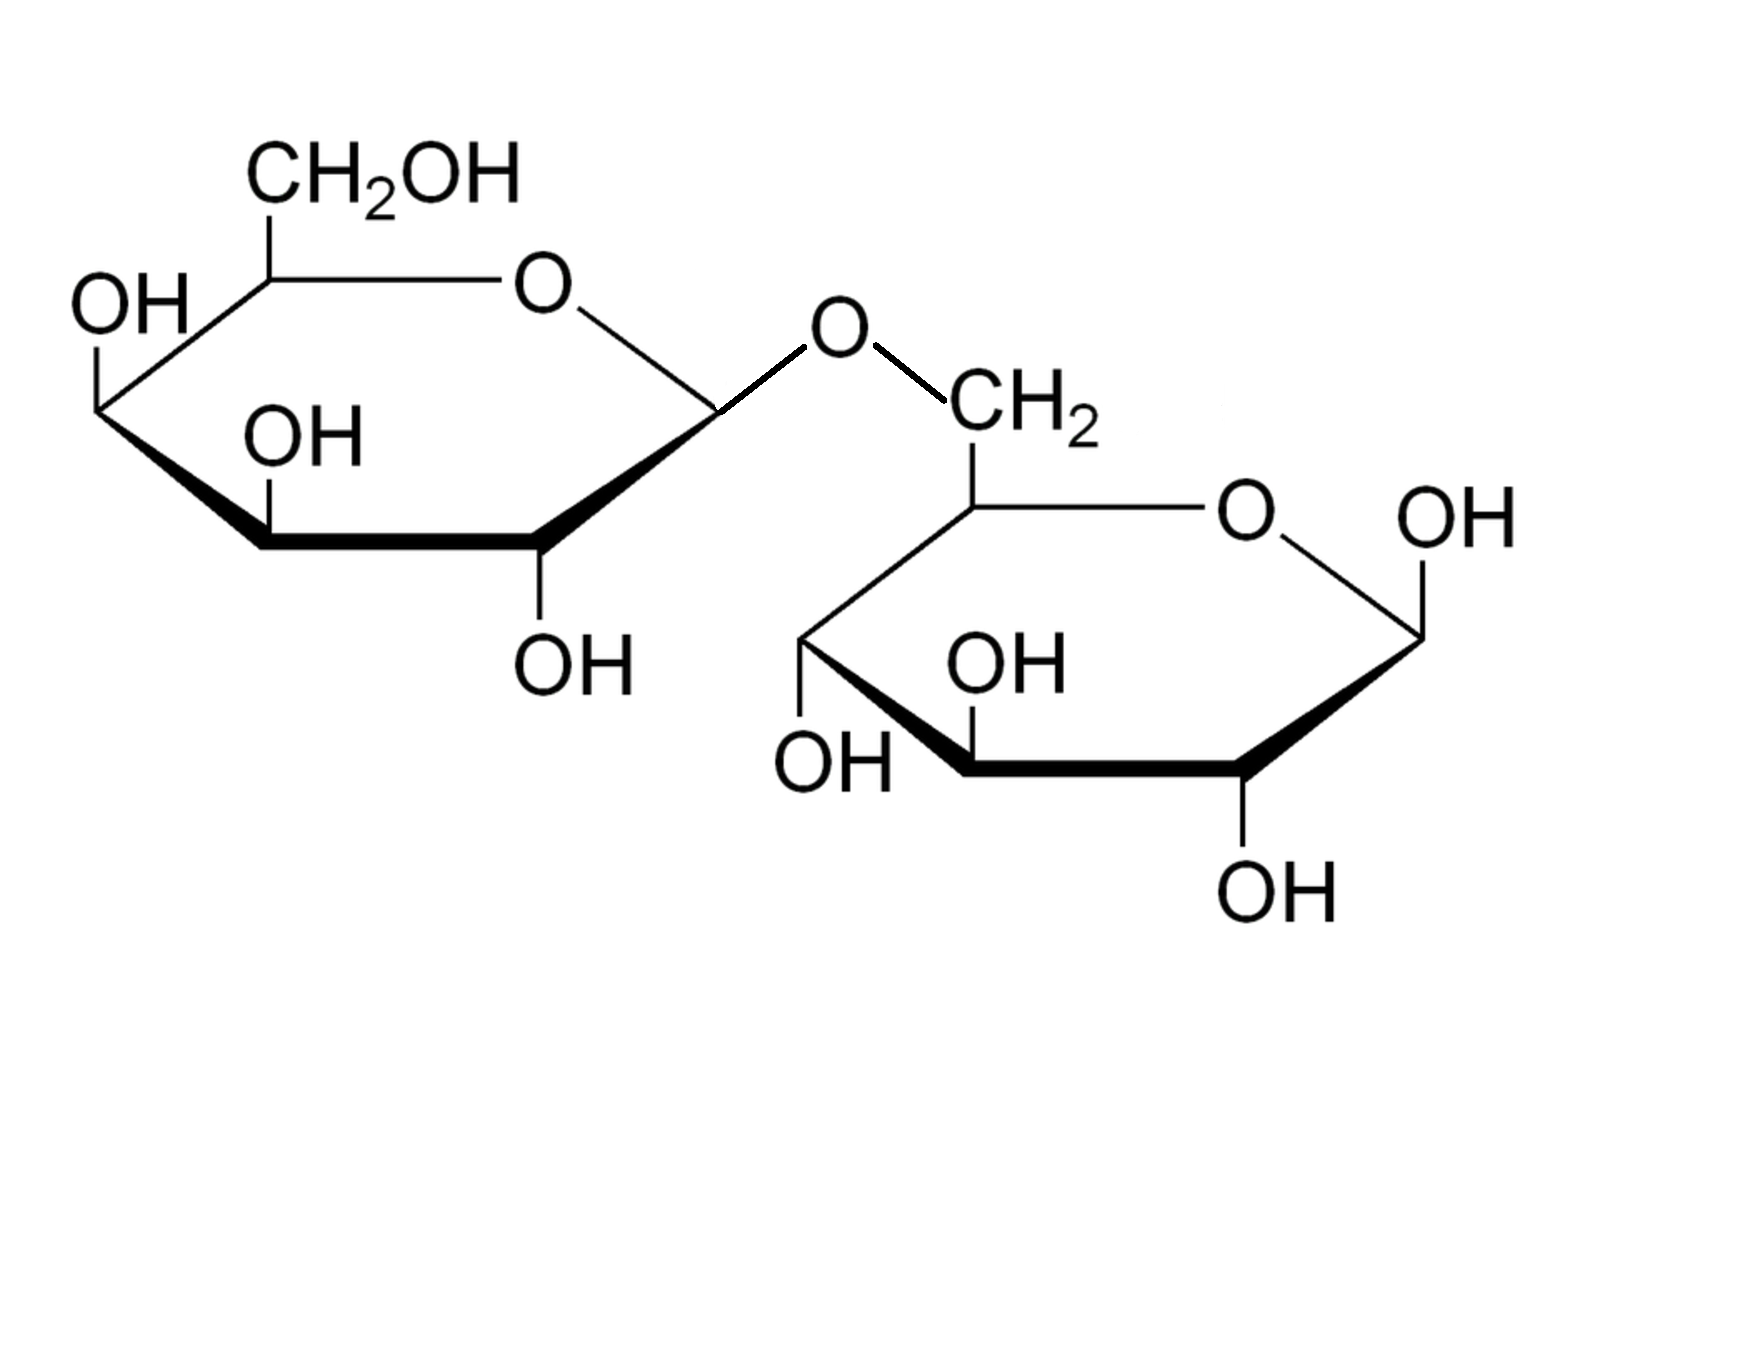
\includegraphics[width=9cm]{./Figures/B-A(1-6)GalactoGlucose.pdf}

\begin{itemize}
\item $\beta$,$\alpha$(1→2)glucofructose
\end{itemize}

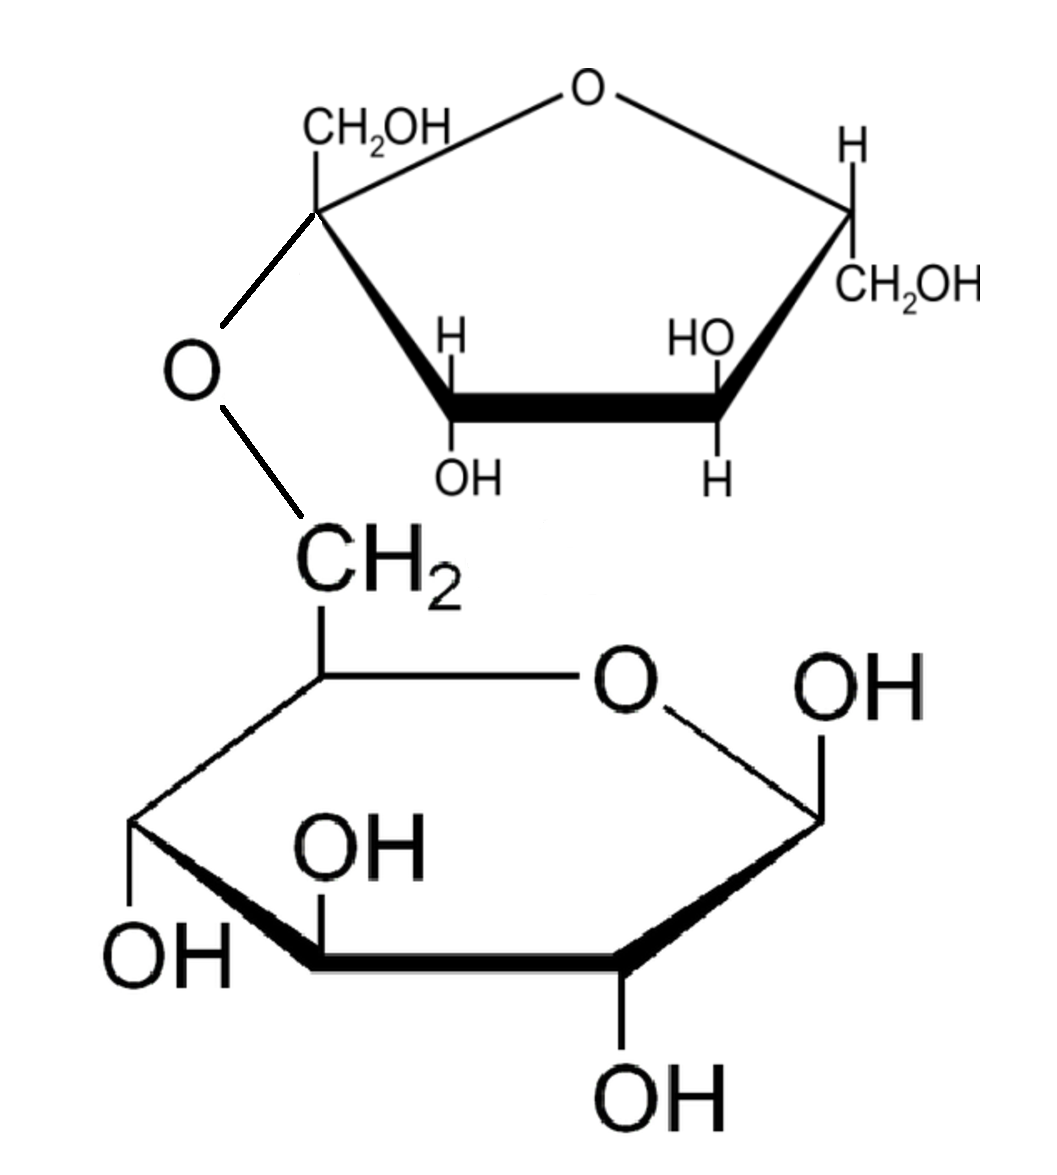
\includegraphics[width=6cm]{./Figures/BA(1-2)GlucoFructose2.pdf}
\section{Questions from Prof. D. De Vos}
\label{sec-3}

Note: reference material for this part mostly come from the
recommended class book \cite{BioChemBlei}

Considering the following molecule:

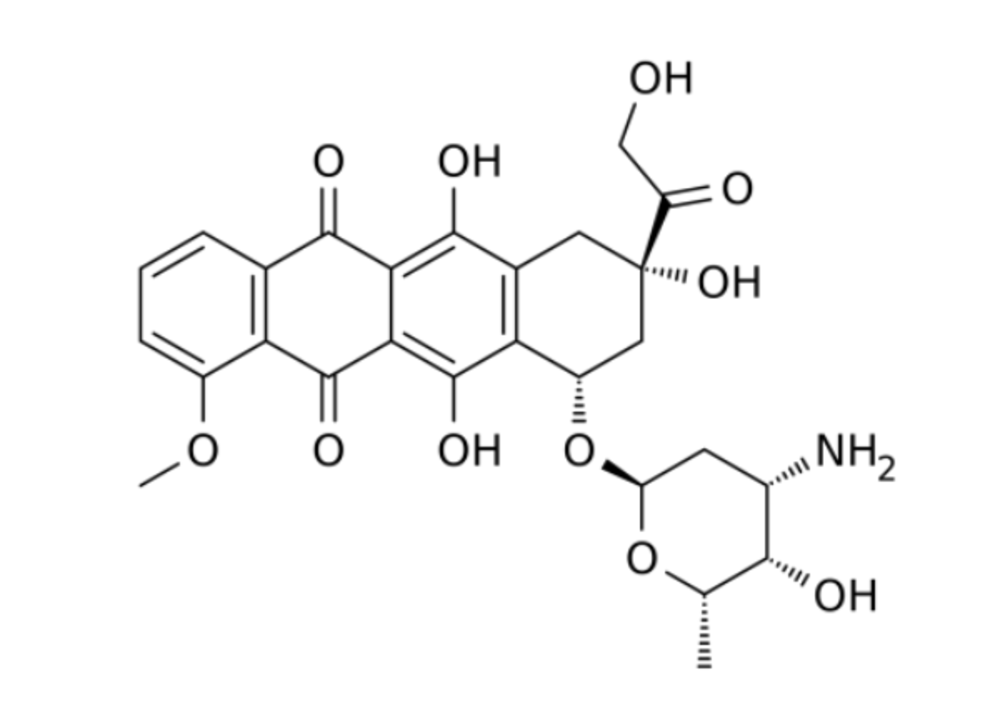
\includegraphics[width=10cm]{./Figures/Part3MoleculeRaw.pdf}
\subsection{Functional groups}
\label{sec-3-1}

\texttt{Q:} Name all functional groups

\texttt{A:} See annoted figure below

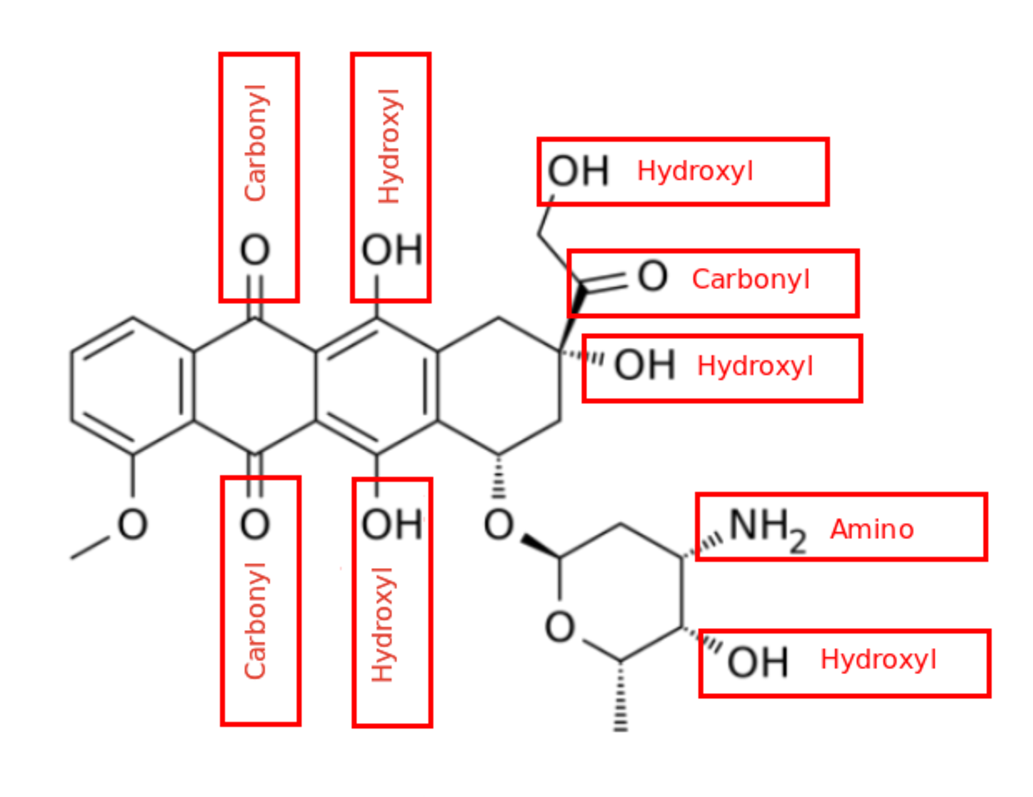
\includegraphics[width=11cm]{./Figures/Part3MoleculeFunctionalGroups.pdf}
\subsection{Water and oil solubility factors}
\label{sec-3-2}

\texttt{Q:} Indicate which groups make the molecule rather water-soluble
than oil-soluble

\texttt{A:} The following groups can partake in hydrogen bonds with water
molecules and increase the solubility of the molecule in water :

\begin{itemize}
\item Hydroxyl groups (5 of them)
\item Carbonyl groups (3 of them)
\item Amino group (1 present)
\end{itemize}


\bibliographystyle{plain}
\bibliography{bib-db}

\end{document}
